% !Mode:: "TeX:UTF-8"
%% 请使用 XeLaTeX 编译本文.
% \documentclass{WHUBachelor}% 选项 forprint: 交付打印时添加, 避免彩色链接字迹打印偏淡. 即使用下一行:
\documentclass[forprint]{WHUBachelor}

% \includeonly{chapter4}

\begin{document}
%%%%%%% 下面的内容, 据实填空.

\miji{ }                                      % 密级. 没有就空着.
\StudentNumber{220205764} % 填写自己的学号

\title{数值分析上机报告 \\ 第五章}
\author{周玉乾}                            % 作者名字
\Cschoolname{微电子学院}          % 学院名
\date{二〇二〇年十二月}                    % 日期, 要注意和英文日期一致!!
\Edate{Nov, 2020}                       % 英文封面日期

%-----------------------------------------------------------------------------
\pdfbookmark[0]{封面}{title}         % 封面页加到 pdf 书签
\maketitle
\frontmatter
\pagenumbering{Roman}              % 正文之前的页码用大写罗马字母编号.
%-----------------------------------------------------------------------------
%% !Mode:: "TeX:UTF-8"

%%% 此部分需要自行填写: (1) 中文摘要及关键词 (2) 英文摘要及关键词
%%%%%%%%%%%%%%%%%%%%%%%%%%%%%
%%% -------------  英文封面 (无需改动)-------------   %%%
%%%%%%%%%%%%%%%%%%%%%%%%%%%%%
\thispagestyle{empty}
\renewcommand{\baselinestretch}{1.5}  %下文的行距
\vspace*{0.5cm}
\begin{center}
{\Large \bf BACHELOR'S DEGREE THESIS \\[1ex] OF WUHAN UNIVERSITY }
\end{center}
\vspace{2.5cm}
\begin{center}{\zihao{2} \the\Etitle \par}\end{center}

\vfill

\begin{center}
\zihao{4}
\begin{tabular}{ r l }
 School (Department): & {\sc \the\Eschoolname}\\
  Major:          &   {\sc\the\Emajor}  \\
 Candidate:      &  {\sc \the\Eauthor}      \\
 Supervisor:     &  {\sc \the\Esupervisor}
\end{tabular}

\vspace*{2cm}
\begin{center}
   \ifprint % 文档打印, 使用黑白校徽.
  \includegraphics[height=4cm]{whu.eps}       %%  黑白的.
  \else
  \includegraphics[height=4cm]{whulogo.eps} %%  彩色的.
  \fi
\end{center}


\zihao{-2}
%\the\Schoolname\\
{\sc Wuhan University}

\vspace*{1.0cm}

\the\Edate

\end{center}
%%% 郑重声明部分无需改动

%%%---- 郑重声明 (无需改动)------------------------------------%
\newpage
\vspace*{20pt}
\begin{center}{\ziju{0.8}\textbf{\songti\zihao{2} 郑重声明}}\end{center}
\par\vspace*{30pt}
\renewcommand{\baselinestretch}{2}

{\zihao{4}%

本人呈交的学位论文, 是在导师的指导下, 独立进行研究工作所取得的成果,
所有数据、图片资料真实可靠. 尽我所知, 除文中已经注明引用的内容外,
本学位论文的研究成果不包含他人享有著作权的内容.
对本论文所涉及的研究工作做出贡献的其他个人和集体,
均已在文中以明确的方式标明. 本学位论文的知识产权归属于培养单位.\\[2cm]

\hspace*{1cm}本人签名: $\underline{\hspace{3.5cm}}$
\hspace{2cm}日期: $\underline{\hspace{3.5cm}}$\hfill\par}
%------------------------------------------------------------------------------
\baselineskip=23pt  % 正文行距为 23 磅
%------------------------------------------------------------------------------





%%======中文摘要===========================%
\begin{cnabstract}
本文主要介绍和讨论了武汉大学本科毕业论文的~\LaTeX~模板.
指明了编译方法, 强调了公式排版的一些细节问题, 也指出了一些常见的排版错误.



\end{cnabstract}
\par
\vspace*{2em}


%%%%--  关键词 -----------------------------------------%%%%%%%%
%%%%-- 注意: 每个关键词之间用“;”分开,最后一个关键词不打标点符号
\cnkeywords{毕业论文; \LaTeX{}; 模板;  }


%%====英文摘要==========================%


\begin{enabstract}
This thesis is a study on the theory of \dots.

\end{enabstract}
\par
\vspace*{2em}

%%%%%-- Key words --------------------------------------%%%%%%%
%%%%-- 注意: 每个关键词之间用“;”分开,最后一个关键词不打标点符号
 \enkeywords{\LaTeX{};  }
    % 加入摘要, 申明.
%==========================把目录加入到书签==============================%%%%%%
%\pdfbookmark[0]{目录}{toc}
%\tableofcontents
\mainmatter %% 以下是正文
%%%%%%%%%%%%%%%%%%%%%%%%%%%--------main matter-------%%%%%%%%%%%%%%%%%%%%%%%%%%%%%%%%%%%%
%\chapter[第一章]{} % (fold)
\label{cha:chapter1}

\section{问题 \\ 舍入误差与有效数字}

设 $S_N = \sum ^N _{j=2} \frac{1}{j^2-1}$,其精确值为 $\frac{1}{2}(\frac{3}{2}-\frac{1}{N}-\frac{1}{N+1})$。

\begin{enumerate}
    \item 编制按从大到小的顺序 $S_N = \frac{1}{2^2-1} + \frac{1}{3^2-1} + ... + \frac{1}{N^2-1}$,计算 $S_N$ 的通用程序;

    \item 编制按从小到大的顺序 $S_N = \frac{1}{N^2-1} + \frac{1}{(N-1)^2-1} + ... + \frac{1}{2^2-1}$,计算 $S_N$ 的通用程序;

    \item 按两种顺序分别计算 $S_{10^2}$、$S_{10^4}$、$S_{10^6}$,并指出其有效位数(编程时用单精度);

    \item 通过本上机题你明白了什么?

\end{enumerate}

\section{分析}

对于 $\frac{1}{N^2-1}$,当 $N$ 很大时,$\frac{1}{N^2-1}$ 接近0,因此如果按从大到小的顺序计算 $S_N = \frac{1}{2^2-1} + \frac{1}{3^2-1} + ... + \frac{1}{N^2-1}$,由于计算机的舍入误差,会出现\textbf{大数吃小数}的情况,从而比真实结果略小;而如果按从小到大的顺序计算 $S_N = \frac{1}{N^2-1} + \frac{1}{(N-1)^2-1} + ... + \frac{1}{2^2-1}$,其结果应该更加接近真实值。

\section{程序}

q1-1.cpp

\begin{lstlisting}[style = cpp]
#include <iostream>
#include <iomanip>
#include <math.h>

float f(int N) {
    float res = 0;
    res = float(1.0)/(pow(float(N), float(2)) - 1);
    return res;
}

float SN_1(int N) {
    float sum = 0;
    for (int i = 2; i <= N; i++)
    {
        sum += f(i);
    }
    return sum;
}

float SN_2(int N) {
    float sum = 0;
    for (int i = N; i >= 2; i--)
    {
        sum += f(i);
    }
    return sum;
}

float SN_Real(int N) {
    float sum = 0;
    sum = 0.5*(1.5 - 1/N - 1/(N+1));
    return sum;
}

int main() {
    float data0 = 0;
    float data1 = 0;
    float data2 = 0;

    int N = 0;

    std::cout<<"请输入N:"<<std::endl;
    std::cin>>N;

    data0 = SN_Real(N);
    data1 = SN_1(N);
    data2 = SN_2(N);

    std::cout<<"N\t精确值\t\t从大到小\t误差1   \t从小到大\t误差2"<<std::endl;
    std::cout<<N<<"\t"<< std::fixed << std::setprecision(8)<<data0<<"\t"<<data1<<"\t"<<abs(data0-data1)<<"\t"<<data2<<"\t"<<abs(data0-data2)<<std::endl;

    return 0;
}
\end{lstlisting}

\section{算例}

\begin{enumerate}
    \item $S_{10^2}$

    \begin{lstlisting}[style = cpp]
$ ./q1-1
请输入N:
100
N   精确值       从大到小      误差1       从小到大      误差2
100 0.75000000  0.74004948  0.00995052  0.74004954  0.00995046
    \end{lstlisting}

    \item $S_{10^4}$

    \begin{lstlisting}[style = cpp]
$ ./q1-1
请输入N:
10000
N       精确值       从大到小      误差1       从小到大      误差2
10000  0.75000000   0.74985212  0.00014788  0.74989998  0.00010002
    \end{lstlisting}

    \item $S_{10^6}$

    \begin{lstlisting}[style = cpp]
$ ./q1-1
请输入N:
1000000
N       精确值       从大到小      误差1       从小到大      误差2
1000000 0.75000000  0.74985212  0.00014788  0.74999905  0.00000095
    \end{lstlisting}

\end{enumerate}

\section{结论}

\begin{table}[ht]
  \centering
  \caption{有效位数}
  \label{tab:1}
  \begin{tabular}{*{20}c}
     \hline
    %  \cline{col1-col2}
     N & $10^2$ & $10^4$ & $10^6$ \\
     \hline
     % after \\: \hline or \cline{col1-col2} \cline{col3-col4} ...
     从大到小 & 1  & 3  & 3 \\
     从小到大 & 1  & 3  & 5 \\
     \hline
   \end{tabular}
\end{table}

\begin{enumerate}
    \item 编程证明了之前的分析,及从大到小求和时,会出现大数吃小数的现象,导致误差偏大;

    \item 再次证明了数学上的等价并不意味着数值上的等价,在实际的运算中,舍入误差的影响不可低估,在计算中选择一种好的算法可以使结果更加精确。
\end{enumerate}



% chapter chapter1 (end)
%\chapter[第二章]{} % (fold)
\label{cha:chapter2}

\section{问题 \\ 试值法或者Newton法同二分法结合}

\subsection{问题1} % (fold)
\label{sub:问题1}

\begin{figure}[ht]
\centering
  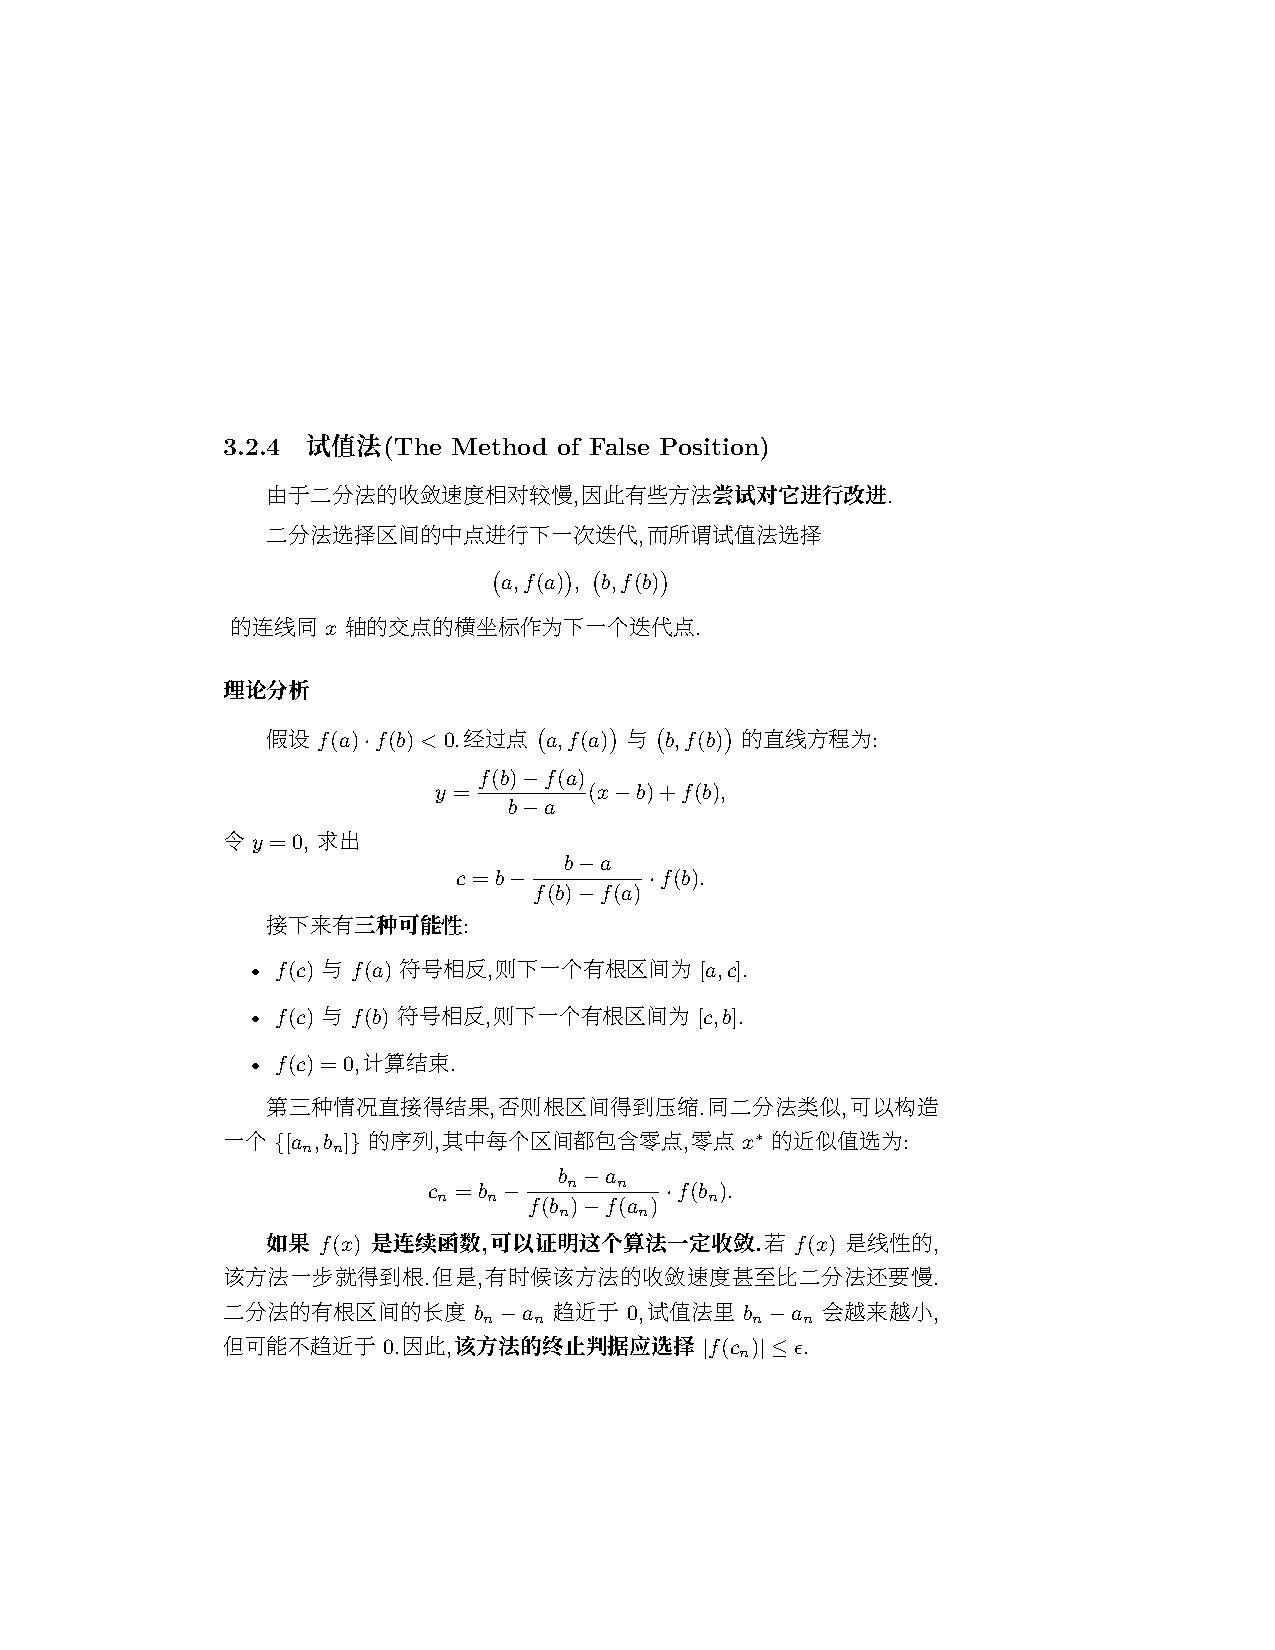
\includegraphics[width=\textwidth]{TVM}
  % \caption{试值法算法}
  % \label{fig:TVM}
\end{figure}

% subsection 问题1 (end)

\subsection{问题2} % (fold)
\label{sub:问题2}

\begin{figure}[ht]
\centering
  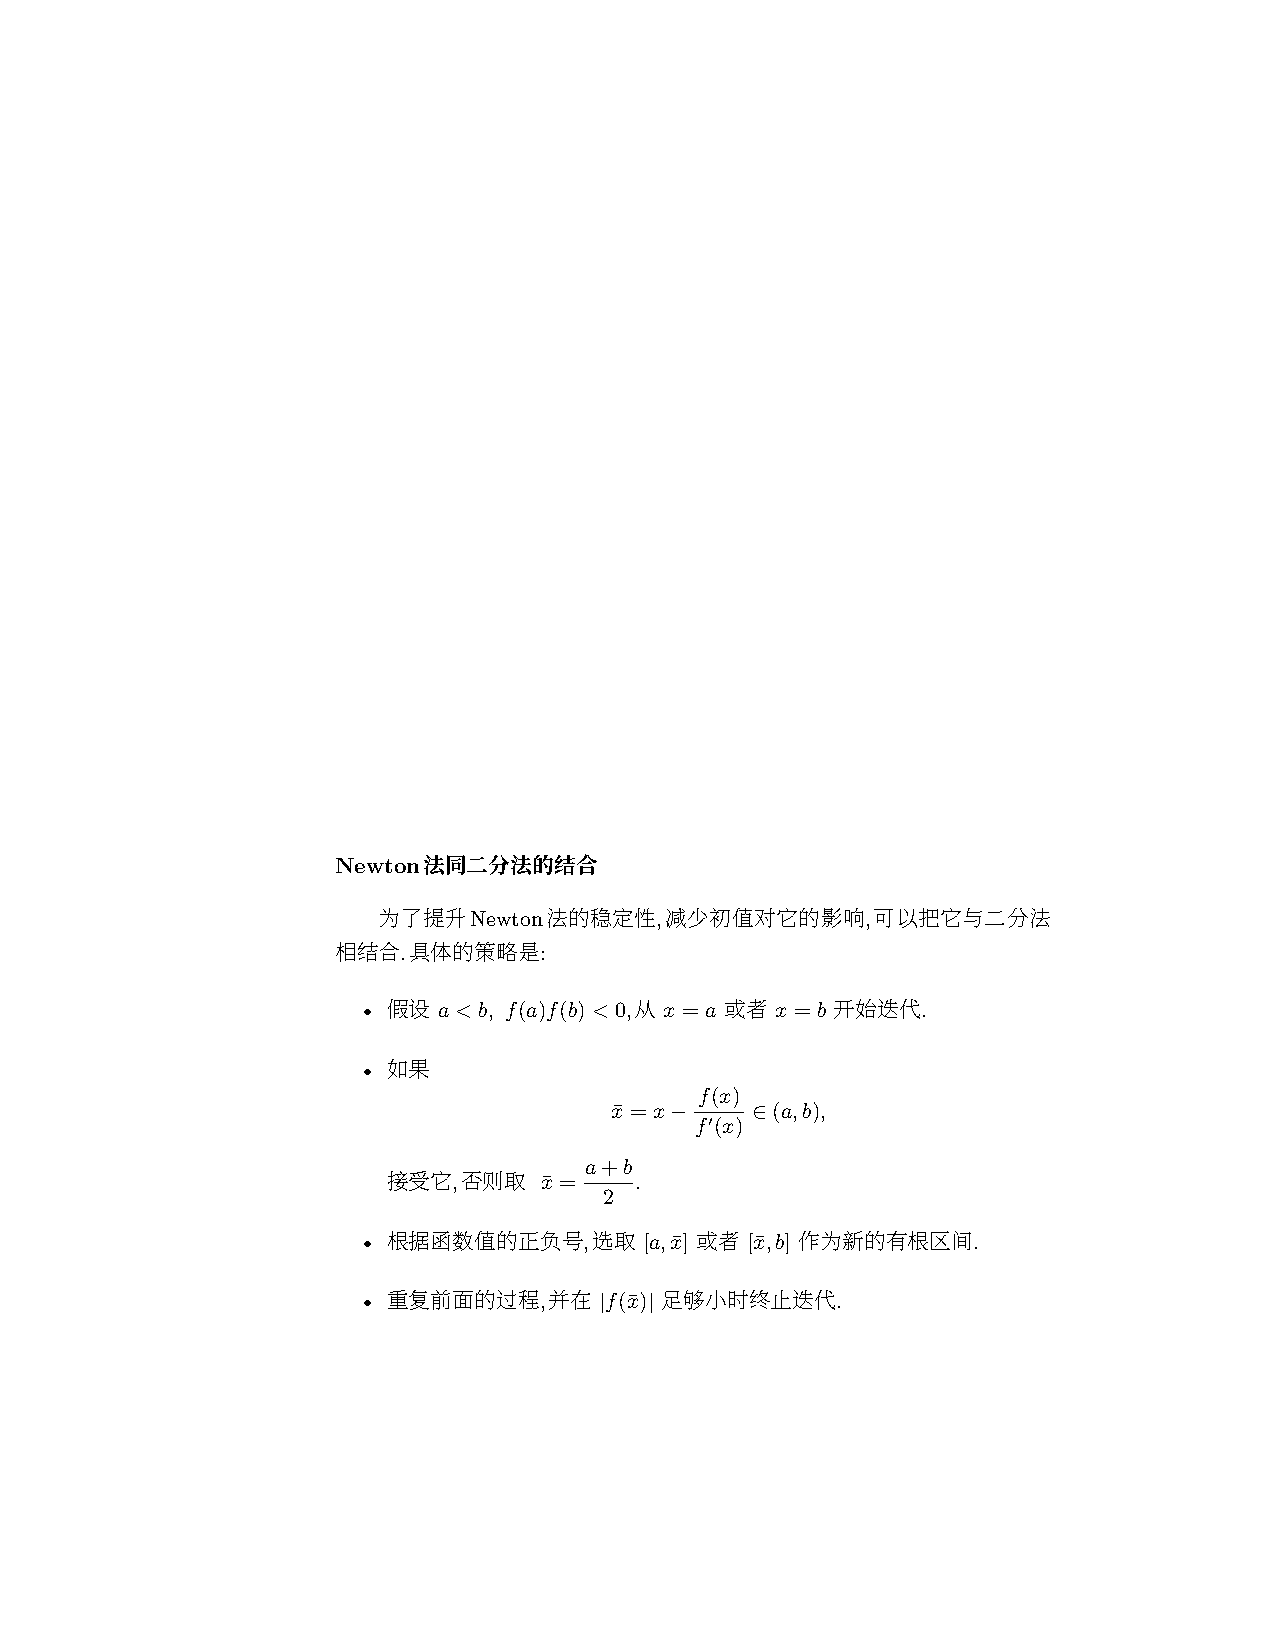
\includegraphics[width=\textwidth]{Newton}
  % \caption{Newton法同二分法结合}
  % \label{fig:Newton}
\end{figure}

% subsection 问题2 (end)


\section{分析}

\subsection{试值法流程}

图\ref{fig:TrailValueFlow} 为试值法算法流程图。

\begin{figure}[ht]
\centering
  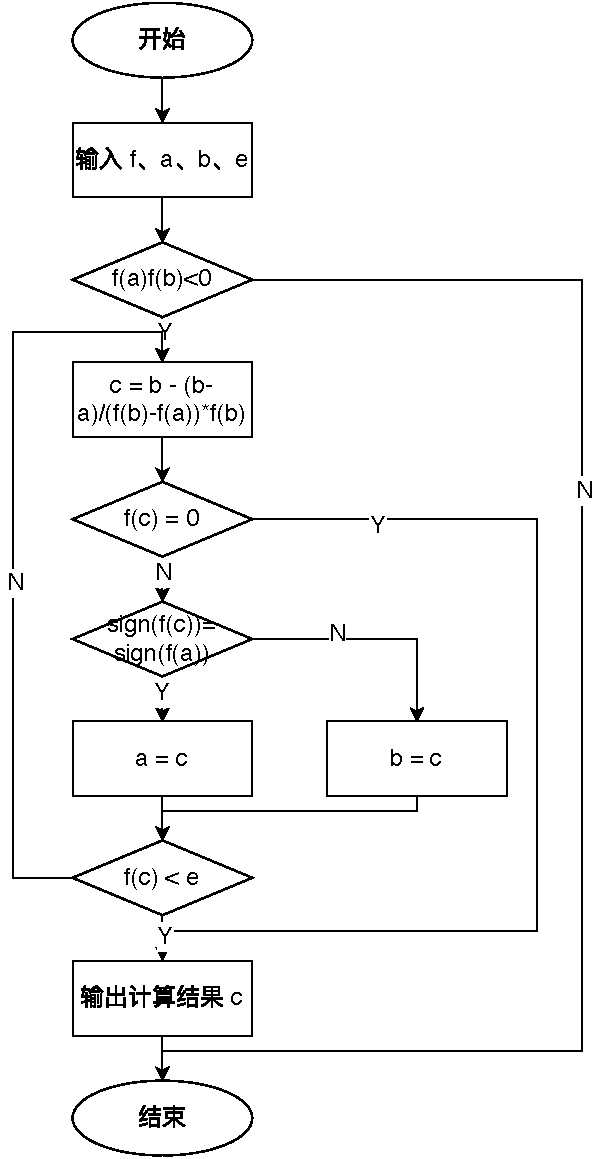
\includegraphics[width=0.5\textwidth]{TrailValueFlow}
  \caption{试值法流程图}
  \label{fig:TrailValueFlow}
\end{figure}

\subsection{Newton法同二分法结合流程}

图\ref{fig:NewtonFlow} 为试值法算法流程图。

\begin{figure}[ht]
\centering
  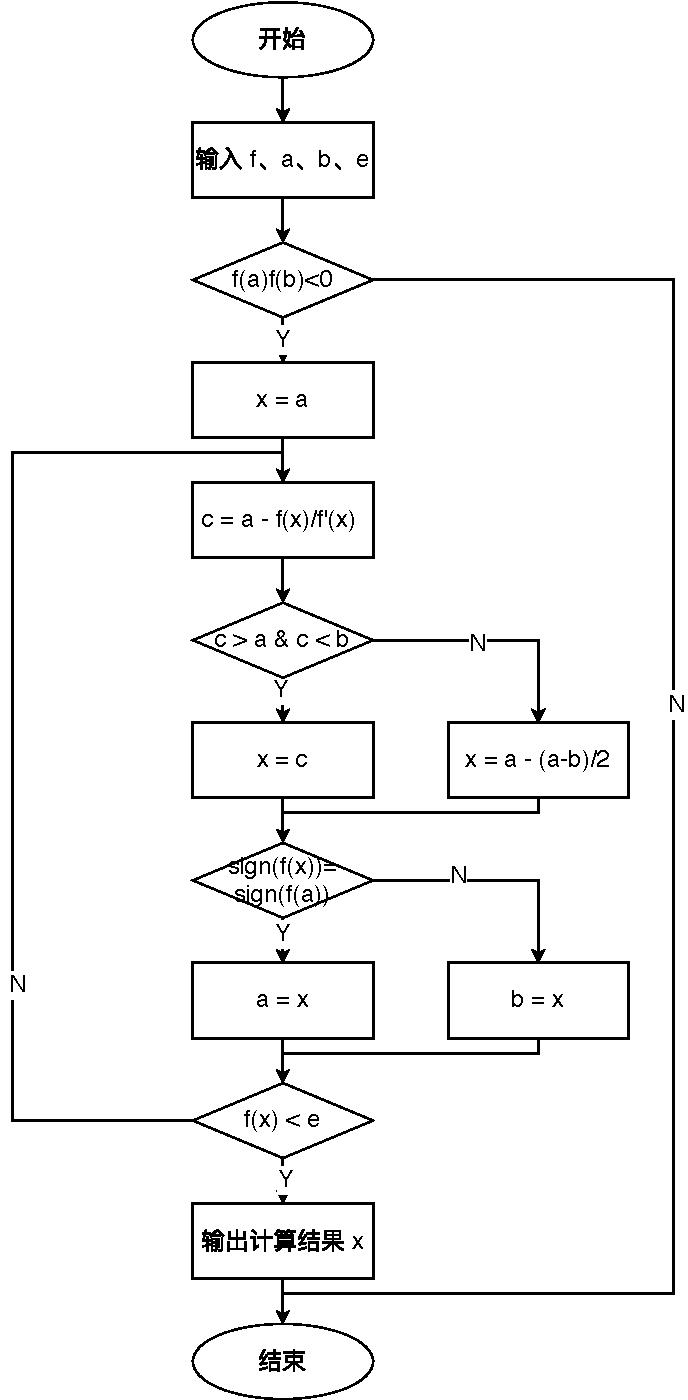
\includegraphics[width=0.5\textwidth]{Newton2Flow}
  \caption{Newton法同二分法结合流程}
  \label{fig:NewtonFlow}
\end{figure}

\section{程序}

试值法

\begin{lstlisting}[style = python]
def TrailValue(expr, a, b, e):
    """
    试值法
    f@函数
    a@区间下限
    b@区间上限
    e@容忍误差限
    """
    f = _func(expr)
    fa_0 = f.value(a)
    fb_0 = f.value(b)
    res = 0
    count = 0
    if abs(fa_0) < e:
        res = a
    elif abs(fb_0) < e:
        res = b
    elif sympy.sign(fa_0) == sympy.sign(fb_0):
        print('f(a) and f(b) 同号')
        sys.exit()
    else:
        while True:
            count = count + 1
            fa = f.value(a)
            fb = f.value(b)
            c = b - ((b-a)/(fb - fa))*fb
            fc = f.value(c)

            # 更新有根区间
            if sympy.sign(fa) == sympy.sign(fc):
                a = c
            else:
                b = c

            # 判断计算结束
            if abs(f.value(c)) < e:
                res = c
                break

    return res, count
\end{lstlisting}

Newton法同二分法结合

\begin{lstlisting}[style = python]
def Newton(expr, a, b, e):
    """
    牛顿法与二分法结合
    f@函数
    a@区间下限
    b@区间上限
    e@容忍误差限
    """
    f = _func(expr)
    fa_0 = f.value(a)
    fb_0 = f.value(b)
    res = 0
    count = 0
    if abs(fa_0) < e:
        res = a
    elif abs(fb_0) < e:
        res = b
    elif sympy.sign(fa_0) == sympy.sign(fb_0):
        print('f(a) and f(b) 同号')
        sys.exit()
    else:
        x = a
        while True:
            count = count + 1
            c = x - f.value(x)/f.diff_value(x)

            # Newton与二分法结合,找下一个点
            if (c > a) and (c < b):
                x = c
            else:
                x = a+(b-a)/2

            # 更新有根区间
            if sympy.sign(f.value(a)) == sympy.sign(f.value(x)):
                a = x
            else:
                b = x

            # 判断计算结束
            if abs(f.value(x)) < e:
                res = x
                break

    return res, count
\end{lstlisting}

\section{算例}

\begin{enumerate}
  \item $x\times sin(x) - 1 = 0$,有根区间为(1, 2),误差限为$1\times 10^{-5}$。

  \begin{lstlisting}[style = python]
  试值法 根: 1.11416, 迭代次数: 3
  牛顿法 根: 1.11416, 迭代次数: 2
  \end{lstlisting}
  
  \item $x^2 - 5 = 0$,有根区间为(2, 3),误差限为$1\times 10^{-5}$。

  \begin{lstlisting}[style = python]
  试值法 根: 2.23607, 迭代次数: 7
  牛顿法 根: 2.23607, 迭代次数: 3
  \end{lstlisting}

  \item $x^3 -3x + 2 = 0$,有根区间为(-2.5, -1.5),误差限为$1\times 10^{-5}$。

  \begin{lstlisting}[style = python]
  试值法 根: -2.00000, 迭代次数: 11
  牛顿法 根: -2.00000, 迭代次数: 4
  \end{lstlisting}

\end{enumerate}

\section{结论}

\begin{enumerate}
  \item 相比于试值法,Newton与二分法结合的算法收敛速度更快;

  \item Newton与二分法结合提升了原始Newton法的稳定性;

  \item 无论是试值法还是Newton与二分法结合的算法,都只能求解函数穿过x轴的根,不能求解函数与x轴相切的根,例如在算例3中,无法求解 $x = 1.0$ 的根。

  \begin{figure}[ht]
  \centering
    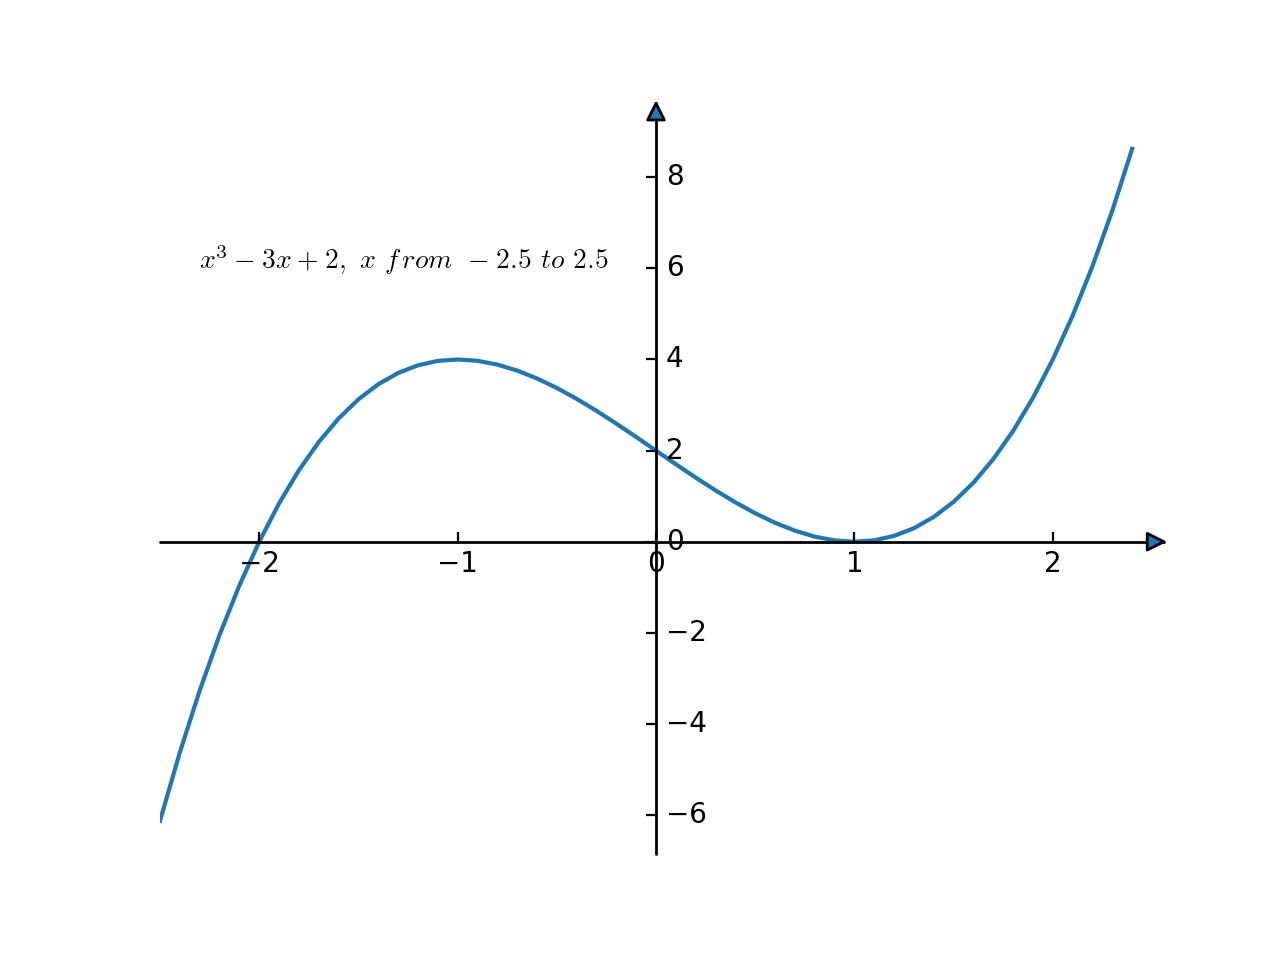
\includegraphics[width=0.6\textwidth]{f3}
    \caption{$f(x) = x^3 -3x + 2$}
    \label{fig:f3}
  \end{figure}

\end{enumerate}

% chapter chapter2 (end)
\setcounter{chapter}{4}
\chapter[第五章]{} % (fold)
\label{cha:chapter5}

\section*{数值积分}

\subsection{问题}

\begin{equation}
    I = \int_0^1 \frac{\mathrm{arctan}x}{x^{\frac{3}{2}}} \mathrm{d}x
\end{equation}



\begin{enumerate}[(1)]
    \item 用 Romberg 公式计算改积分,使误差不超过 $\frac{1}{2}\times 10^{-7}$;
    \item ⽤复化 3 点 Gauss-Legendre 公式计算它,使误差不超过 $\frac{1}{2}\times 10^{-7}$。
\end{enumerate}

\subsection{分析}

\subsubsection{复化 Romberg 公式的分析}

\begin{enumerate}[(1)]
    \item 首先用递推关系求梯形公式:
    \begin{align}
        T_1 &= h(\frac{1}{2}f(a)+\frac{1}{2}f(b)) \\
        T_{2n} &= \frac{1}{2}T_n + \frac{h(n)}{2}\sum\nolimits_{n=0}^{n-1}f(x_{k+1/2})
    \end{align}

    \item 利用梯形公式求 Simpson 公式:
    \begin{equation}
        S_n(f) = \frac{4}{3}T_{2n}(f) - \frac{1}{3}T_n(f)
    \end{equation}

    \item 利用 Simpson 公式求 Cotes 公式:
    \begin{equation}
        C_n(f) = \frac{16}{15}S_{2n}(f)-\frac{1}{15}S_n(f)
    \end{equation}

    \item 最后用 Cotes 求 Romberg 公式:
    \begin{equation}
        R_n(f) = \frac{64}{63}C_{2n}(f)-\frac{1}{63}C_n(f)
    \end{equation}
\end{enumerate}

\subsubsection{Gauss-Legendre 求积公式分析}

\begin{enumerate}[(1)]
    \item $[-1,1]$ 上的3点Gauss-Legendre公式:
    \begin{equation}
        \int_{-1}^1 g(x)\mathrm{d}x \approx \frac{5}{9}g(-\sqrt{\frac{3}{5}}) + \frac{8}{9}g(0) + \frac{5}{9}g(\sqrt{\frac{3}{5}})
    \end{equation}

    \item 一般区间 $[a,b]$ 上的 Gauss 公式:
    
    令 $x_k = \frac{a+b}{2}+\frac{b-a}{2}t_k$,$A_k = \frac{b-a}{2}\tilde{A}_k$,$k=0:n$

    \item 由于 Gauss 求积公式的节点不具有递推性,因此考虑用截断误差计算节点的数量, Gauss-Lengdre 公式的截断误差为:
    \begin{multline}
        R(f) = \int _a^b f(x)\mathrm{d}x - \sum\nolimits_{k=0}^n A_kf(x_k) = \frac{f^{2n+2}(\xi)}{(2n+2)!} \int_a^b W_{n+1}^2(x)\mathrm{d}x, \\
        W_{n+1}(x) = \prod\nolimits_{j=0}^n (x-x_j), \quad \xi \in (a,b)
    \end{multline}

    由于导数计算不太方便,并且还需要求函数的最大值,增加了程序的复杂性。考虑到使用分段积分可以极大地减少计算量(后面结论分析会给出一个分段与不分段计算时间的对比),因此用每次将区间长度减小一半,计算出一个 $R_n(f)$,用前后两次结果的差值作为误差判断的依据(后验误差),只要误差小于误差限,就停止计算。

\end{enumerate}

\subsubsection{待积函数分析}

待求积分的函数为:

\begin{equation}
    g(x) = \frac{\mathrm{arctan}x}{x^{3/2}}
\end{equation}

该函数的图像如图\ref{fig:f}所示,是一个奇异函数,在 $x=0$ 处有奇异点,值为 $+\infty$,用 Romberg 公式求积时需要用到 $x=0$ 处的值。在 $[0,x_0]$ 上的积分用右矩形公式的两倍近似,即 $\int_0^{x_0} g(x) \mathrm{d}x \approx 2\cdot x_0 \cdot g(x_0) $,保证近似值小于一半的误差限,即 $2\cdot x_0 \cdot g(x_0) \leq 1/2 \times 1/2 \times 10^{-7}$;

为了减少计算量,在 $[x_0, 1]$ 上,做分段积分,分别对 $[x_0,1\times 10^{-9}]$、$[1\times 10^{-9},1\times 10^{-4}]$、$[1\times 10^{-4},1]$做Romberg积分,每一段的误差都要求小于 $1/6 \times 1/2 \times 10^{-7}$,这样保证总的误差不超过 $ 1/2 \times 10^{-7}$。

\begin{figure}[ht]
    \centering
      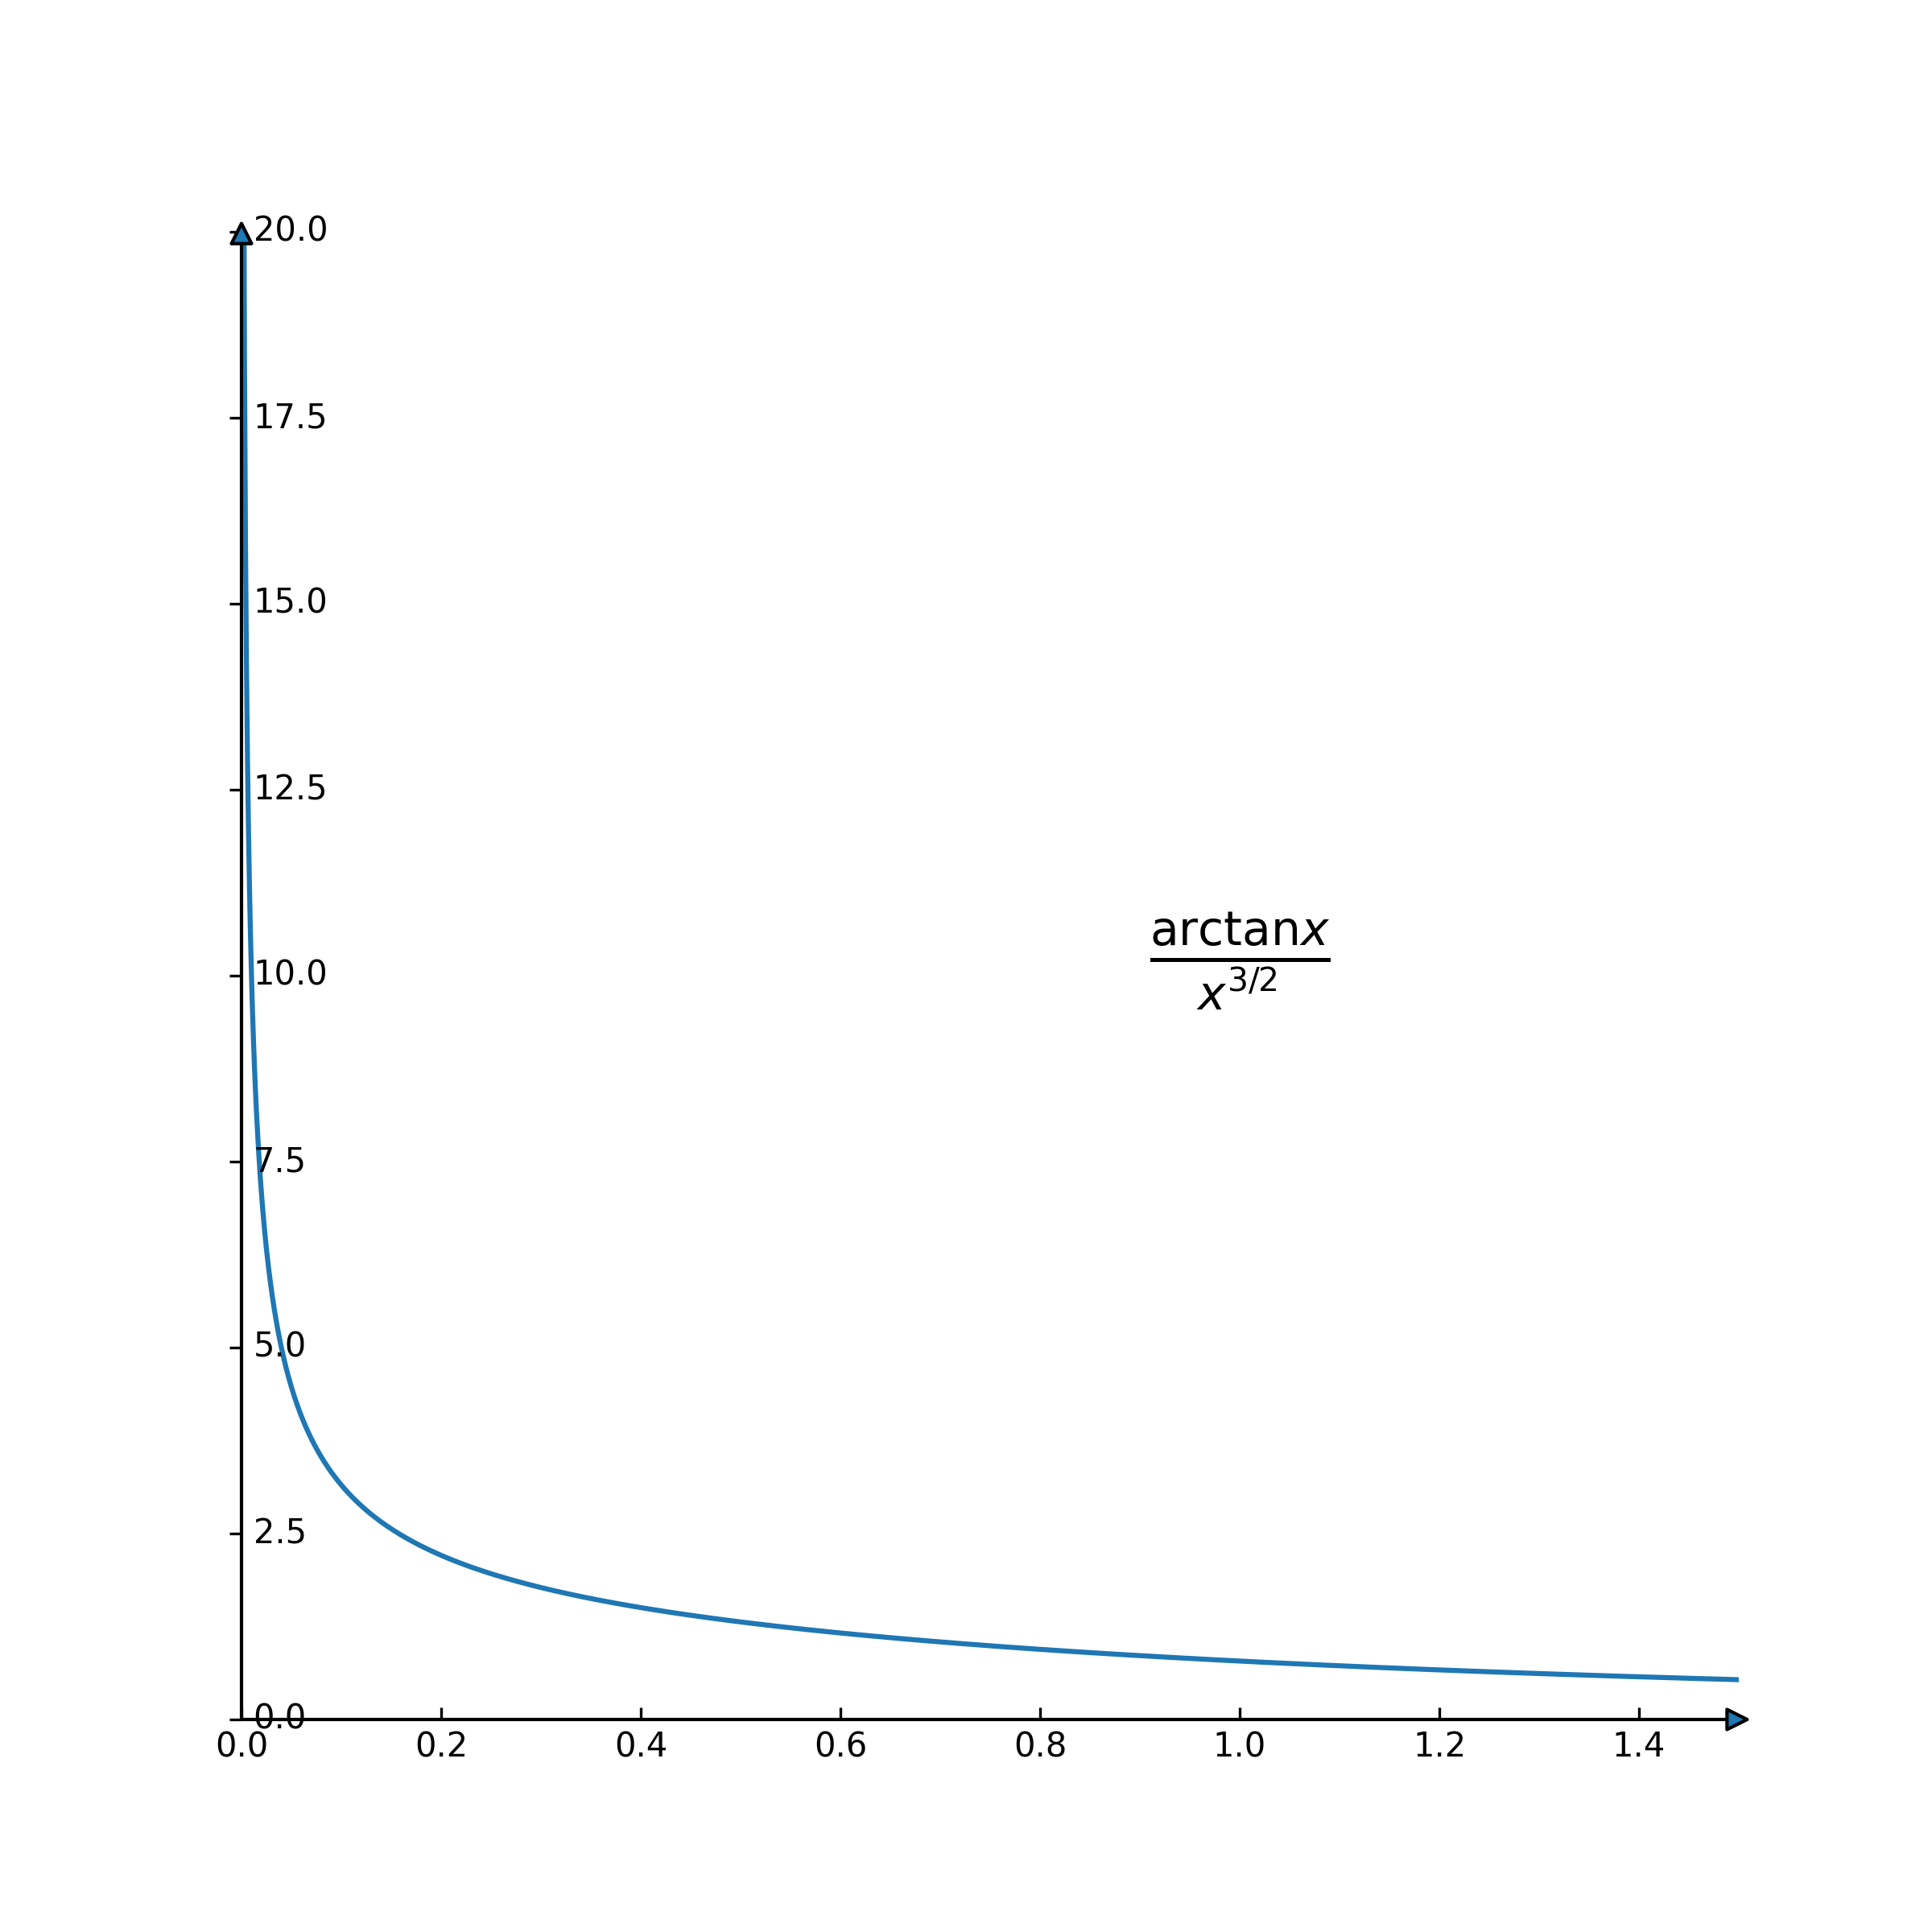
\includegraphics[width=0.5\textwidth]{fq3}
      \caption{$(\mathrm{arctan}x)/(x^{3/2})$ 图像}
      \label{fig:f}
\end{figure}

\subsection{程序}

\subsubsection{q3\_romberg.py}

\begin{lstlisting}[style = python]
    import math
    import time
    import os, sys
    
    RESULT_FILE = os.path.join(os.path.dirname(os.path.abspath(__file__)), 'q3_romberg_result.txt')
    
    def print_row(lst, n):
        print('n =: ', n, ', ',' '.join('%11.8f, ' % x for x in lst))
        with open(RESULT_FILE, "a+") as fo:
            fo.write('n: {0}, '.format(n))
            for x in lst:
                fo.write('{0}, '.format(x))
            fo.write('\n')
    
    
    def romberg(f, a, b, eps=1e-8):
        """Approximate the definite integral of f from a to b by Romberg's method.
        eps is the desired accuracy."""
        R = [[0.5 * (b - a) * (f(a) + f(b))]]  # R[0][0]
        print_row(R[0], 1)
        n = 1
        while True:
            h = float(b - a) / 2 ** n
            R_row_tmp = []
            R_row_tmp_0 = 0.5*R[n-1][0] + h*sum(f(a+(2*k-1)*h) for k in range(1, 2**(n-1)+1))
            R_row_tmp.append(R_row_tmp_0)
            for m in range(1, min(n, 3)+1):
                tmp = R_row_tmp[m-1] + (R_row_tmp[m-1] - R[n-1][m-1]) / (4 ** m - 1)
                R_row_tmp.append(tmp)
            R.append(R_row_tmp)
            print_row(R[n], 2**n)
            if n >= 4 and abs(R[n-1][3] - R[n][3])/255.0 < eps:
                return R[n][-1]
            n += 1
    
    '''
    description: 处理反常积分奇异点为 0 的情况,返回
    return {*} 
    '''
    def Improper_deal(f, a, b, err=1e-8):
        m = 2
        x = a + (b-a)/m
        while 2.0*f(x)*x > err:
            m = m * 2.0
            x = a + (b-a)/m
        return x
    
    def expression0(x):
        return 1.0/x
    
    def expression1(x):
        return math.atan(x)/(pow(x, 1.5))
    
    def main():
        a = Improper_deal(expression1, 0, 1, (0.5e-7)/2.0)
        print(a)
        with open(RESULT_FILE, "a+") as fo:
            fo.write('a = {0}, '.format(a))
            fo.write('\n')
        print('int3')
        int3 = romberg(expression1, 1e-4, 1, (0.5e-7)/6.0) # 
        print('int2')
        int2 = romberg(expression1, 1e-9, 1e-4, (0.5e-7)/6.0) #
        print('int1')
        int1 = romberg(expression1, a, 1e-9, (0.5e-7)/100.0) # 100.0
        int_all = int1+int2+int3
        print('result is {0} .'.format(int_all))
        with open(RESULT_FILE, "a+") as fo:
            fo.write('n: {0}, '.format(int_all))
            fo.write('\n')
    
    
    if __name__ == "__main__":
        time_start = time.time()
        if os.path.exists(RESULT_FILE):
            os.remove(RESULT_FILE)
        main()
        time_end=time.time()
        print('time cost {0} s. '.format(time_end - time_start))
        with open(RESULT_FILE, "a+") as fo:
            fo.write('time cost {0} s. \n'.format(time_end - time_start))
\end{lstlisting}

\subsubsection{q3\_gauss\_legendre.py}

\begin{lstlisting}[style = python]
    import time
    import math
    import os, sys
    
    RESULT_FILE = os.path.join(os.path.dirname(os.path.abspath(__file__)), 'q3_gauss_legendre_result.txt')
    
    def Gauss_Legendre(f, a, b):
        Int = (b-a) * (5.0 * f(0.5*(a+b-(b-a)*pow(3.0/5.0, 0.5))) + \
            8.0 * f(0.5*(a+b)) + 5.0 * f(0.5*(a+b+(b-a)*(pow(3.0/5.0, 0.5))))) / (9.0*2.0)
        return Int
    
    def Com_Gauss_Legendre(f, a, b, n):
        h = (b-a)/n
        Int_Sum = 0.0
        for i in range(1, n+1):
            x0 = a + (i - 1.0) * h
            x1 = a + i * h
            Int_Sum += Gauss_Legendre(f, x0, x1)
        return Int_Sum
    
    def Get_Com_Gauss_Legendre(f, a, b, err):
        Int_Last = 0
        i = 0
        while True:
            Int = Com_Gauss_Legendre(f, a, b, 2 ** i)
    
            print('n: {0}, {1}'.format(2**i, Int))
            with open(RESULT_FILE, "a+") as fo:
                fo.write('n: {0}, {1} \n'.format(2**i, Int))
    
            if abs(Int - Int_Last) <= err:
                return Int, i
            else:
                Int_Last = Int
                i += 1
    
    def expression1(x):
        return math.atan(x)/(pow(x, 1.5))
    
    def main():
        print('int3')
        int3, n3 = Get_Com_Gauss_Legendre(expression1, 1e-5, 1, (0.5e-7)/6.0) # 
        print('int2')
        int2, n2 = Get_Com_Gauss_Legendre(expression1, 1e-10, 1e-5, (0.5e-7)/6.0) #
        print('int1')
        int1, n1 = Get_Com_Gauss_Legendre(expression1, 0, 1e-10, (0.5e-7)/6.0) # 100.0
        int_all = int1+int2+int3
        n_times = 2**(n1+n2+n3)
        print('result is {0} , n is {1}'.format(int_all, n_times))
        with open(RESULT_FILE, "a+") as fo:
            fo.write('result is {0} , n is {1}'.format(int_all, n_times))
            fo.write('\n')
    
    if __name__ == "__main__":
        time_start = time.time()
        if os.path.exists(RESULT_FILE):
            os.remove(RESULT_FILE)
        main()
        time_end=time.time()
        print('time cost {0} s. '.format(time_end - time_start))
        with open(RESULT_FILE, "a+") as fo:
            fo.write('time cost {0} s. \n'.format(time_end - time_start))
\end{lstlisting}

\subsection{算例}

\begin{equation}
    I = \int_0^1 \frac{\mathrm{arctan}x}{x^{\frac{3}{2}}} \mathrm{d}x
\end{equation}

分段的考虑是分3段,调整3段的长度,尽量使每一段上面的计算次数相等,这样应该可以使总的计算次数最少。

用 Romberg 求积公式的实际积分区间是$[1.110223025\times 10^{-16},1\times 10^{-9}]$、$[1\times 10^{-9},1\times 10^{-4}]$、$[1\times 10^{-4},1]$,计算出来的结果是:$1.897097415$;

用 Gauss-Legendre 求积公式实际积分区间是$[0,1\times 10^{-10}]$、$[1\times 10^{-10},1\times 10^{-5}]$、$[1\times 10^{-5},1]$,计算出来的结果是:$1.897095603$。

\subsection{结论}

算术解的结果为(使用\href{https://www.wolframalpha.com/}{wolframalpha.com}计算):
\begin{multline}
    y = -\frac{log(x - \sqrt{2x} + 1)}{\sqrt{2}} + \frac{log(x + \sqrt{2x} + 1)}{\sqrt{2}} {} \\
    - \sqrt{2} tan^{-1}(1 - \sqrt{2x}) + \sqrt{2} tan^{-1}(\sqrt{2x} + 1) - \frac{2 tan^{-1}(x)}{\sqrt{x}}
\end{multline}

因此准确解是:$1.897095623$。

\subsubsection{复化 Romberg 公式}

对比准确解可以看到,实际误差为$1.8\times 10^{-6}$,大于所要求的的 $\frac{1}{2}\times 10^{-7}$,且计算值略大于真实值,分析后应该是在 $[x_0,1\times 10^{-9}]$ 这段上误差太大,因为在 $x_0$ 处的值还是太大了,因此将这段的误差设为 $1/2\times 10^{-9}$,其他两段的误差设定保持 $1/6 \times 1/2 \times 10^{-7}$,再次计算出来的结果是 $1.897095976$,误差是 $3.5\times 10^{-7}$,达到了误差的要求。

在没有分段积分时,程序跑了一周多也没有收敛到误差要求内,在设定好合适的分段积分区间后,程序只运行了 0.2 s 就收敛到误差要求内,效率提升很大。

\subsubsection{Gauss-Legendre 求积公式}

对比准确解可以看到,使用分段后的 Gauss-Legendre 求积公式计算结果的误差为 $2.0\time 10^{-8}$,达到了误差的要求。

与Romberg求积类似,在没有分段积分时,程序跑了一周多也没有收敛到误差要求内,在设定好合适的分段积分区间后,程序只运行了 1.9 s 就收敛到误差要求内,效率提升很大。

\subsubsection{总结}

计算奇异函数,分段计算很有必要,可以极大地减少计算量,提高计算速度。

\footnote{所有的代码和tex格式的报告见\href{https://github.com/Starrynightzyq/SEU-NumericalAnalysis-Exercises.git}{https://github.com/Starrynightzyq/SEU-NumericalAnalysis-Exercises}}
% chapter chapter5 (end)


%%%-------------- 附录. 不需要可以删除.-----------
\appendix

%\chapter{第二章代码}

q2-1.py

\begin{lstlisting}[style = python]
import sys
import sympy

def func_1_expr():
    """
    x*sin(x) - 1 = 0
    """
    x = sympy.symbols('x')
    return x*sympy.sin(x)-1.0

def func_2_expr():
    """
    x^2 - 5 = 0
    """
    x = sympy.symbols('x')
    return x**2.0 - 5.0

def func_3_expr():
    """
    x^3 -3x + 2 = 0
    """
    x = sympy.symbols('x')
    return x**3.0 - 3.0*x +2

class _func():
    """
    计算一元函数值及导数值
    """
    def __init__(self, expr, eff=15):
        """
        初始化计算表达式
        expr@表达式
        eff@有效数字位数
        """
        self._expr = expr()
        self._eff = eff
        self._x = list(self._expr.free_symbols)[0]
        self._diff_expr = sympy.diff(self._expr, self._x)

    def value(self, x):
        """
        计算 func 值
        """
        expr = self._expr
        return expr.subs('x', x).evalf(self._eff)

    def diff_value(self, x):
        """
        计算导数值
        """
        expr = self._diff_expr
        return expr.subs('x', x).evalf(self._eff)

          

def TrailValue(expr, a, b, e):
    """
    试值法
    f@函数
    a@区间下限
    b@区间上限
    e@容忍误差限
    """
    f = _func(expr)
    fa_0 = f.value(a)
    fb_0 = f.value(b)
    res = 0
    count = 0
    if abs(fa_0) < e:
        res = a
    elif abs(fb_0) < e:
        res = b
    elif sympy.sign(fa_0) == sympy.sign(fb_0):
        print('f(a) and f(b) 同号')
        sys.exit()
    else:
        while True:
            count = count + 1
            fa = f.value(a)
            fb = f.value(b)
            c = b - ((b-a)/(fb - fa))*fb
            fc = f.value(c)

            # 更新有根区间
            if sympy.sign(fa) == sympy.sign(fc):
                a = c
            else:
                b = c

            # 判断计算结束
            if abs(f.value(c)) < e:
                res = c
                break

    return res, count

def Newton(expr, a, b, e):
    """
    牛顿法与二分法结合
    f@函数
    a@区间下限
    b@区间上限
    e@容忍误差限
    """
    f = _func(expr)
    fa_0 = f.value(a)
    fb_0 = f.value(b)
    res = 0
    count = 0
    if abs(fa_0) < e:
        res = a
    elif abs(fb_0) < e:
        res = b
    elif sympy.sign(fa_0) == sympy.sign(fb_0):
        print('f(a) and f(b) 同号')
        sys.exit()
    else:
        x = a
        while True:
            count = count + 1
            c = x - f.value(x)/f.diff_value(x)

            # Newton与二分法结合,找下一个点
            if (c > a) and (c < b):
                x = c
            else:
                x = a+(b-a)/2

            # 更新有根区间
            if sympy.sign(f.value(a)) == sympy.sign(f.value(x)):
                a = x
            else:
                b = x

            # 判断计算结束
            if abs(f.value(x)) < e:
                res = x
                break

    return res, count
        
def main():
    """
    main
    """
    res_t, count_t = TrailValue(func_1_expr, 1, 2, 1.0/sympy.Pow(10, 5))
    print('试值法 func 1 根: %.5f, 迭代次数: %d' % (res_t, count_t))

    res_n, count_n = Newton(func_1_expr, 1, 2, 1.0/sympy.Pow(10, 5))
    print('牛顿法 func 1 根: %.5f, 迭代次数: %d' % (res_n, count_n))

    res_t, count_t = TrailValue(func_2_expr, 2, 3, 1.0/sympy.Pow(10, 5))
    print('试值法 func 2 根: %.5f, 迭代次数: %d' % (res_t, count_t))

    res_n, count_n = Newton(func_2_expr, 2, 3, 1.0/sympy.Pow(10, 5))
    print('牛顿法 func 2 根: %.5f, 迭代次数: %d' % (res_n, count_n))

    res_t, count_t = TrailValue(func_3_expr, -2.5, -1.5, 1.0/sympy.Pow(10, 5))
    print('试值法 func 3 根: %.5f, 迭代次数: %d' % (res_t, count_t))

    res_n, count_n = Newton(func_3_expr, -2.5, -1.5, 1.0/sympy.Pow(10, 5))
    print('牛顿法 func 3 根: %.5f, 迭代次数: %d' % (res_n, count_n))

if __name__ == "__main__":
    main()
\end{lstlisting}

\cleardoublepage
\end{document}



